\documentclass[12pt]{article}
\usepackage[margin=1in]{geometry}
\usepackage{graphicx}
\usepackage{booktabs}
\usepackage{hyperref}
\usepackage{titlesec}
\usepackage{enumitem}
\usepackage{fancyvrb}
\usepackage{float}

\title{MILS Assignment I Report}
\author{Ian Ku}
\date{}

\begin{document}

\maketitle
\noindent\textbf{GitHub Repository:} \url{https://github.com/IanKu304/2025S_DL_HW1_RE6131066_Ianku}
\section*{Dataset}
The mini-ImageNet dataset was used for all experiments. It consists of 50 classes with training, validation, and test sets defined in \texttt{train.txt}, \texttt{val.txt}, and \texttt{test.txt}. All images were resized to 32x32 or 224x224 as appropriate for the network architecture.

\section*{Problem A: Dynamic Convolution Module}

\subsection*{Design Objective}
We designed a convolutional module that:
\begin{itemize}[noitemsep]
    \item Handles arbitrary input channels (e.g., RGB, RG, R)
    \item Is spatial size invariant
    \item Dynamically generates convolution kernels
\end{itemize}

\section*{Training Configuration}

All models were trained using the same training protocol to ensure fair comparison. The key hyperparameters and strategies are summarized below:

\begin{itemize}
    \item \textbf{Optimizer:} Adam optimizer with an initial learning rate of $1 \times 10^{-3}$
    \item \textbf{Loss Function:} Cross-Entropy Loss for multi-class classification
    \item \textbf{Batch Size:} 10
    \item \textbf{Max Epochs:} 40 epochs
    \item \textbf{Early Stopping:} Enabled, with a patience of 5 epochs based on validation loss in Section A and 10 in Section B
    \item \textbf{Learning Rate Scheduler:} Not used
    \item \textbf{Input Size:}
    \begin{itemize}
        \item $32 \times 32$ for DynamicCNN and BaselineCNN (Problem A)
        \item $224 \times 224$ for ResNet34 and custom 2/4-layer CNNs (Problem B)
    \end{itemize}
    \item \textbf{Channel Robustness:} For Problem A, optional \texttt{RandomChannelDrop} was used with probability 0.3 to simulate partial channel inputs (e.g., RG, R)
    \item \textbf{Weight Initialization:} PyTorch default initialization
\end{itemize}

\subsection*{Architectures}

\subsubsection*{DynamicCNN v1}
\begin{Verbatim}
Input Channels: 1–3
→ MLP (input channel as condition) → Dynamic Kernel
→ Conv2D → BN → ReLU → GAP → FC(32→50)
\end{Verbatim}

\subsubsection*{DynamicCNN v2}
\begin{Verbatim}
Input Channels: 1–3
→ CNN-based kernel generator → Dynamic Kernel
→ Conv2D → BN → ReLU 
→ Conv(32→64) → BN → ReLU → GAP 
→ FC(64→128) → ReLU → FC(128→50)
\end{Verbatim}

\subsubsection*{Baseline CNN}
\begin{Verbatim}
Conv(3→32, 3x3) → ReLU → BN → MaxPool
Conv(32→64, 3x3) → ReLU → BN → GAP
FC(64→50)
\end{Verbatim}

\subsection*{Results on Test Set (32x32)}

\textbf{Without Channel Dropout:}
\begin{center}
\begin{tabular}{lccc}
\toprule
Model & Accuracy & FLOPs & Params \\
\midrule
DynamicCNN v1 & 0.2422 & 180.39 KMac & 31.57 K \\
DynamicCNN v2 & 0.1422 & 19.49 MMac & 63.31 K \\
Baseline CNN & 0.2844 & 5.95 MMac & 22.83 K \\
\bottomrule
\end{tabular}
\end{center}

\begin{figure}[H]
\centering
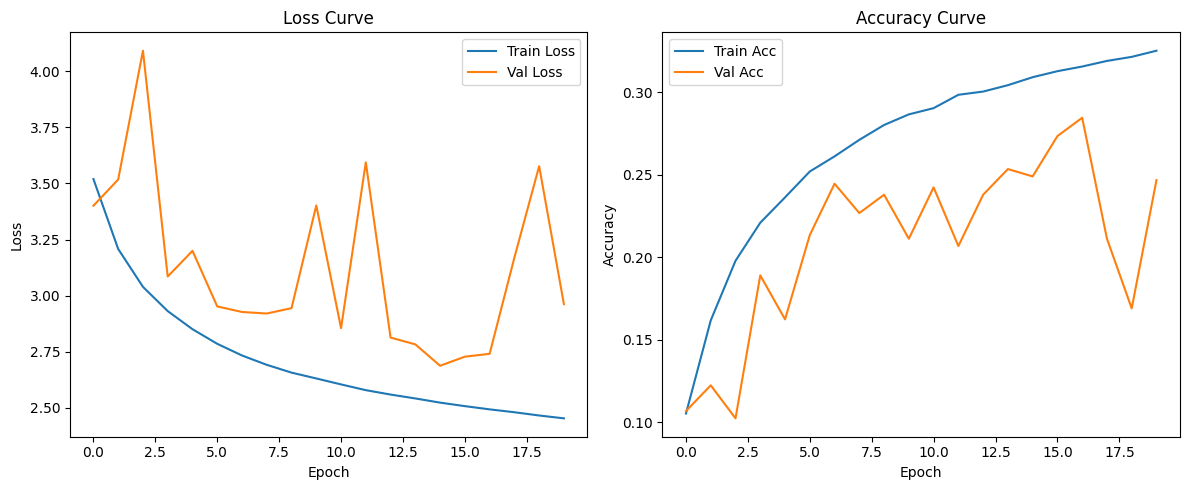
\includegraphics[width=0.8\linewidth]{results/Baseline_CNN_no_drop.png}
\caption{Training plot for Baseline CNN  without random channel drop}
\end{figure}

\begin{figure}[H]
\centering
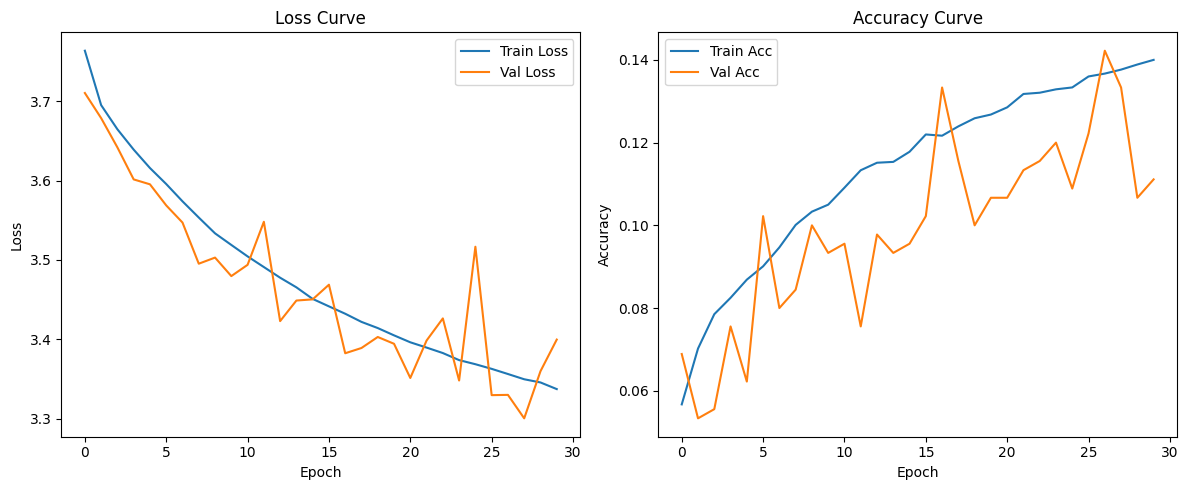
\includegraphics[width=0.8\linewidth]{results/Dynamic1_no_drop.png}
\caption{Training plot for DynamicCNN v1 without random channel drop}
\end{figure}

\begin{figure}[H]
\centering
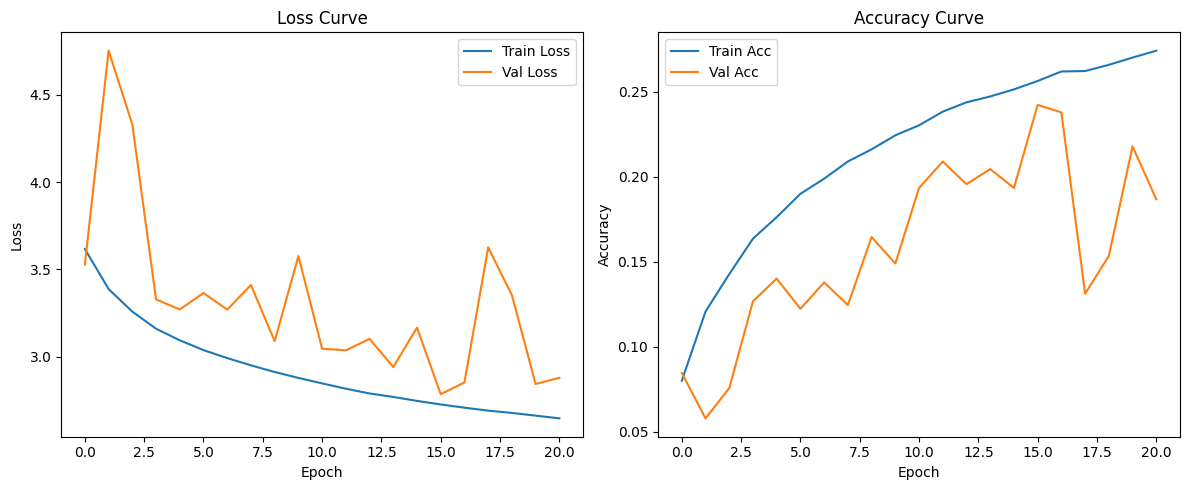
\includegraphics[width=0.8\linewidth]{results/Dynamic2_no_drop.png}
\caption{Training plot for DynamicCNN v without random channel drop}
\end{figure}


\textbf{With RandomChannelDrop:}
\begin{center}
\begin{tabular}{lccc}
\toprule
Model & Accuracy & FLOPs & Params \\
\midrule
DynamicCNN v1 & 0.1244 & 180.39 KMac & 31.57 K \\
DynamicCNN v2 & 0.2244 & 19.49 MMac & 63.31 K \\
Baseline CNN & 0.2422 & 5.95 MMac & 22.83 K \\
\bottomrule
\end{tabular}
\end{center}


\begin{figure}[H]
\centering
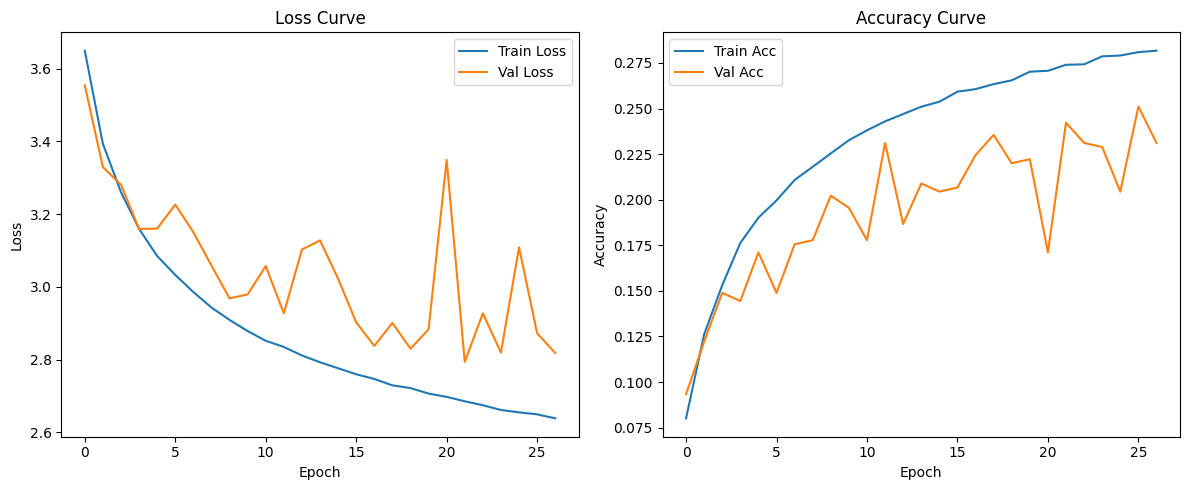
\includegraphics[width=0.8\linewidth]{results/Baseline_CNN_drop.png}
\caption{Training plot for Baseline CNN  with random channel drop}
\end{figure}

\begin{figure}[H]
\centering
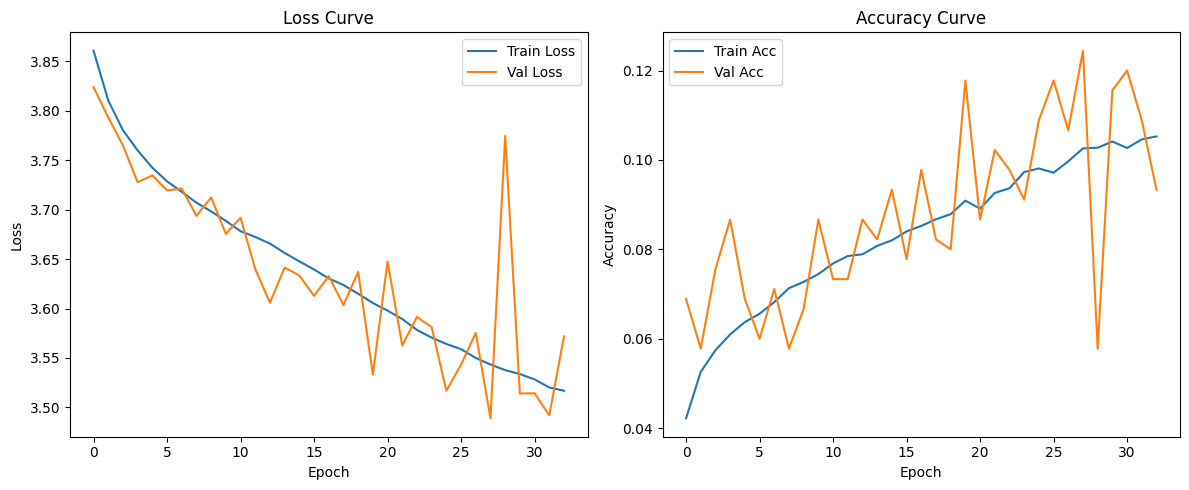
\includegraphics[width=0.8\linewidth]{results/Dynamic1_drop.png}
\caption{Training plot for DynamicCNN v1 with random channel drop}
\end{figure}

\begin{figure}[H]
\centering
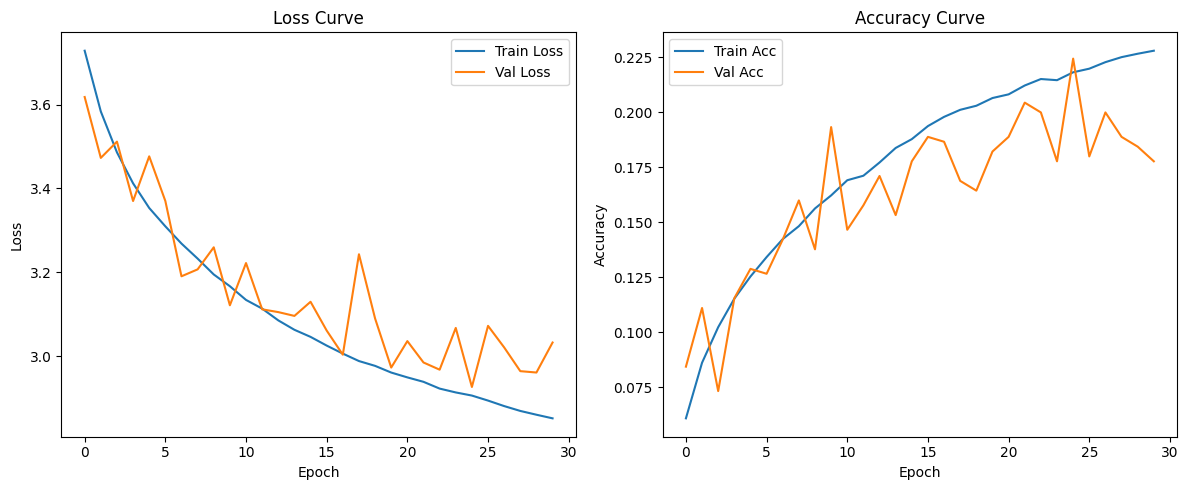
\includegraphics[width=0.8\linewidth]{results/Dynamic2_drop.png}
\caption{Training plot for DynamicCNN v2 with random channel drop}
\end{figure}

\section*{Problem B: Two-Layer Network}

\subsection*{Design Goal}
Design a 2--4 effective layer network achieving at least 90\% of ResNet34's performance on mini-ImageNet (resized to 224x224).

\subsection*{Architectures}

\subsubsection*{ResNet34 (baseline)}
\begin{Verbatim}
Input → Conv(7x7, 64) → MaxPool
[3x BasicBlock(64)]
[4x BasicBlock(128)]
[6x BasicBlock(256)]
[3x BasicBlock(512)]
→ GAP → FC(50)
\end{Verbatim}

\subsubsection*{Simple2LayerCNN}
\begin{Verbatim}
Conv(3→32, 7x7) → BN → ReLU
Conv(32→64, 5x5) → BN → ReLU → SEBlock(64) → MaxPool
Conv(64→128, 5x5) → BN → ReLU → SEBlock(128) → GAP
FC(128→128) → ReLU → FC(128→50)
\end{Verbatim}

\subsubsection*{Simple4LayerCNN}
\begin{Verbatim}
Conv(3→32, 3x3) → BN → ReLU
Conv(32→64, 3x3) → BN → ReLU
Conv(64→128, 3x3) → BN → ReLU
Conv(128→128, 3x3) → BN → ReLU
GAP → FC(128→128) → ReLU → FC(128→50)
\end{Verbatim}

\subsection*{Results (224x224)}

\begin{center}
\begin{tabular}{lcccc}
\toprule
Model & Accuracy & FLOPs & Params & Train Time \\
\midrule
ResNet34 & 0.5667 & 3.68 GMac & 21.31 M & 234.85 min \\
Simple2LayerCNN & 0.4400 & 43.66 MMac & 237.75 K & 451.15 min \\
Simple4LayerCNN & 0.4000 & 285.83 MMac & 301.11 K & 470.57 min \\
SE2LayerCNN & 0.4711 & 43.82 MMac & 240.51 K & 843.25 min \\
\bottomrule
\end{tabular}
\end{center}





\begin{figure}[H]
\centering
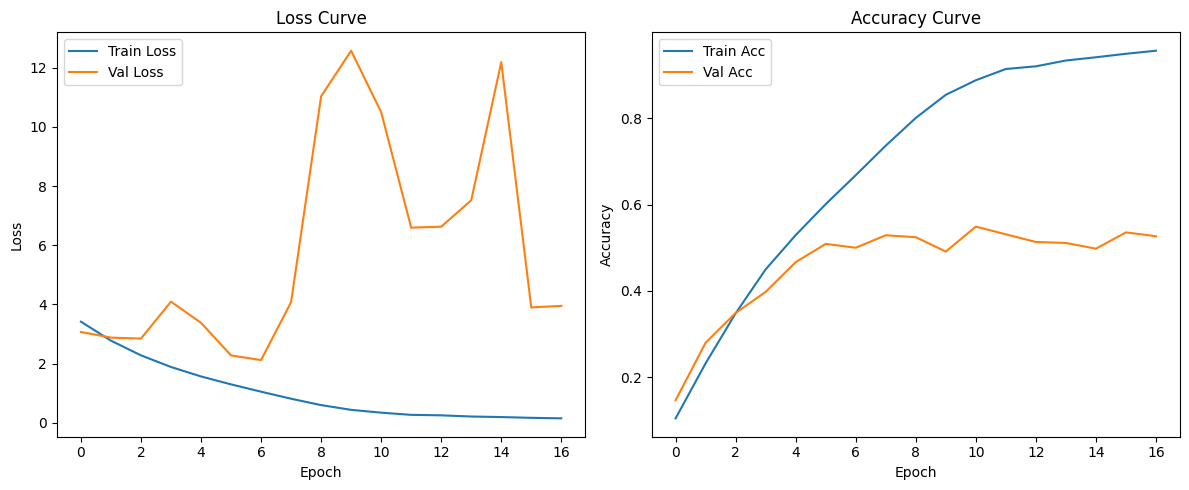
\includegraphics[width=0.8\linewidth]{results/ResNet34.png}
\caption{Training plot for ResNet34 model}
\end{figure}

\begin{figure}[H]
\centering
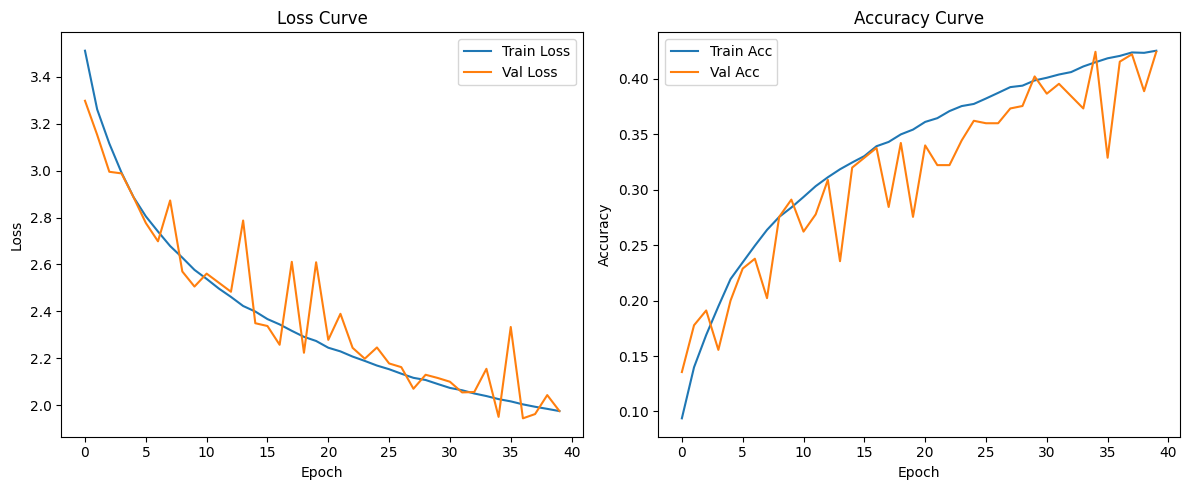
\includegraphics[width=0.8\linewidth]{results/Attention1.png}
\caption{Training plot 1 for Attention model}
\end{figure}


\begin{figure}[H]
\centering
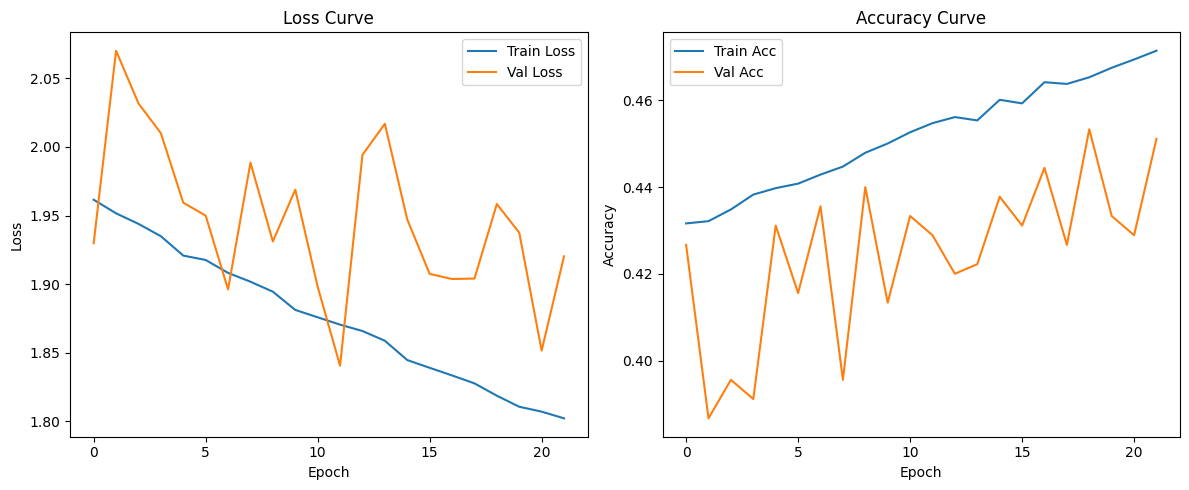
\includegraphics[width=0.8\linewidth]{results/Attention2.png}
\caption{Training plot 2 for Attention model}
\end{figure}

\begin{figure}[H]
\centering
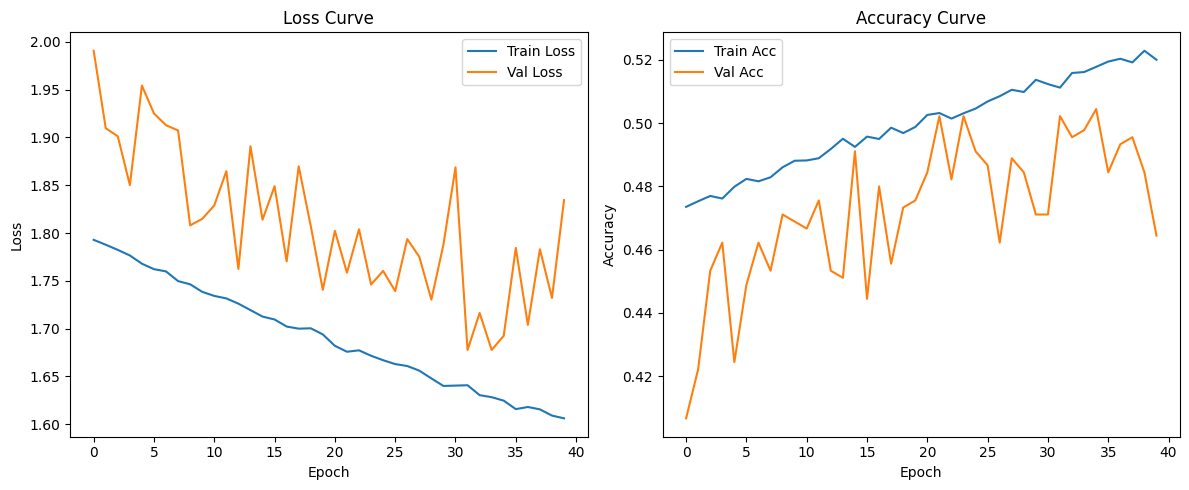
\includegraphics[width=0.8\linewidth]{results/Attention3.png}
\caption{Training plot 3 for Attention model}
\end{figure}

\begin{figure}[H]
\centering
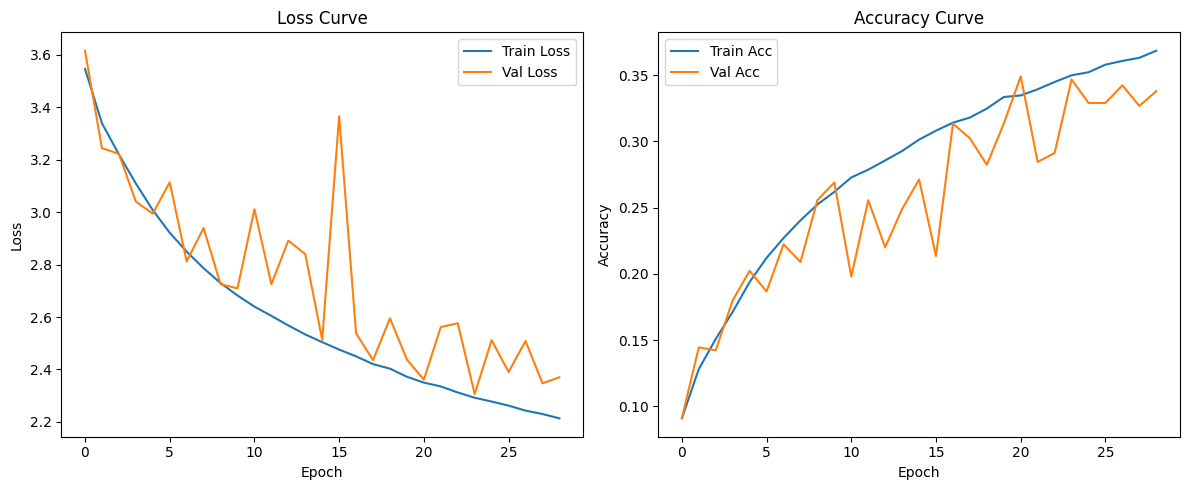
\includegraphics[width=0.8\linewidth]{results/S2CNN_1.png}
\caption{Training plot 1 for S2CNN}
\end{figure}


\begin{figure}[H]
\centering
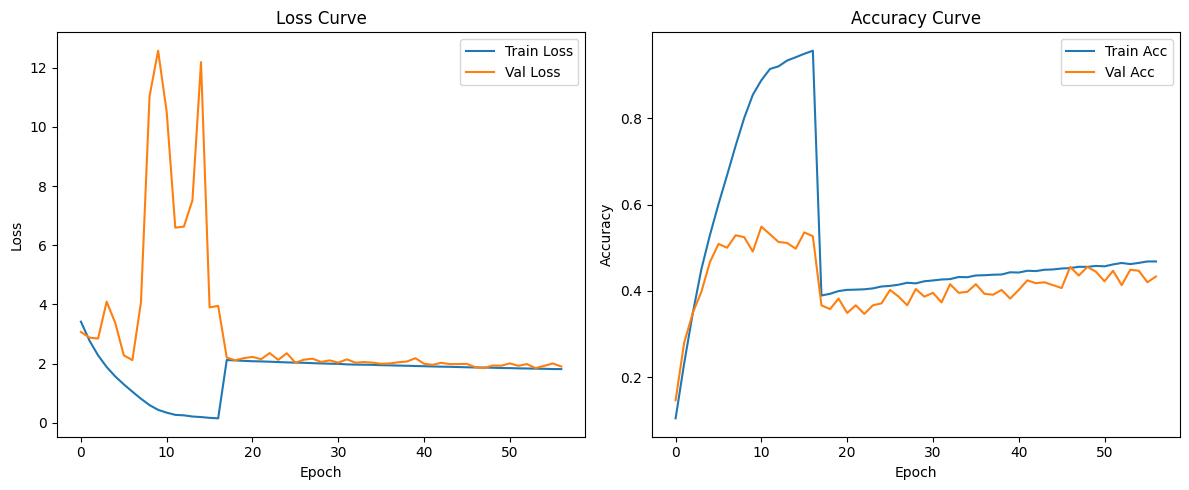
\includegraphics[width=0.8\linewidth]{results/S2CNN_2.png}
\caption{Training plot 2 for S2CNN}
\end{figure}


\begin{figure}[H]
\centering
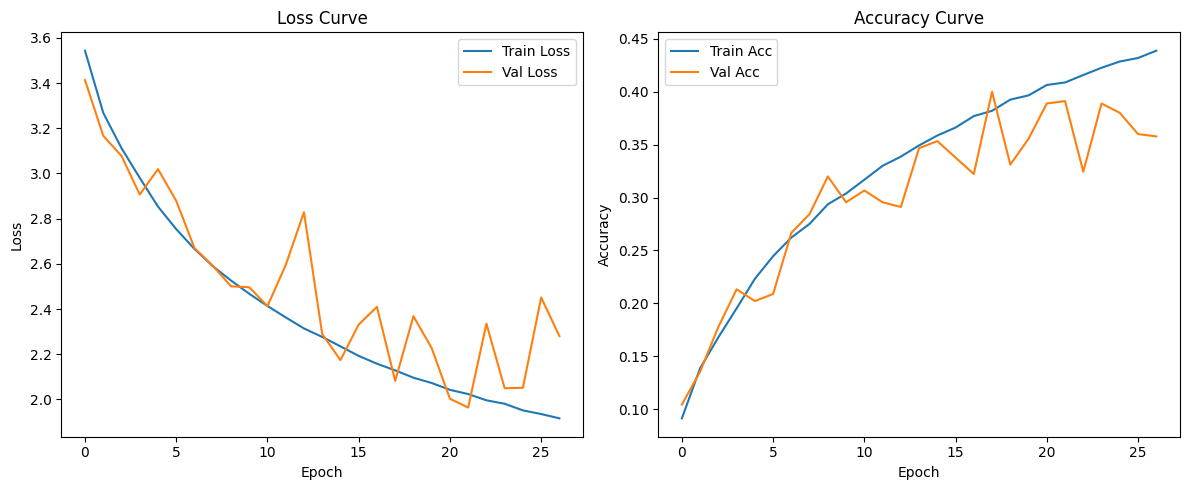
\includegraphics[width=0.8\linewidth]{results/S4CNN.png}
\caption{Training plot for S4CNN}
\end{figure}



\section*{Summary and Insights}

\subsection*{Problem A}
\begin{itemize}[noitemsep]
    \item \textbf{DynamicCNN v1} achieves best result without channel dropout.
    \item \textbf{DynamicCNN v2} is more robust under channel variation.
    \item \textbf{BaselineCNN} provides stable performance overall.
\end{itemize}

\subsection*{Problem B}
\begin{itemize}[noitemsep]
    \item \textbf{Simple2LayerCNN} achieves 77.6\% of ResNet34.
    \item \textbf{SE2LayerCNN} boosts accuracy with minor cost.
    \item \textbf{Simple4LayerCNN} deeper model did not improve performance.
\end{itemize}

\section*{Appendix}




\end{document}